\documentclass[12pt]{article}
\usepackage{amsmath}
\usepackage{graphicx}
\usepackage{hyperref}
\usepackage{listings}
\usepackage{xcolor}
\usepackage{physics}
\usepackage{natbib}

\lstset{
    language=Python,
    basicstyle=\ttfamily\small,
    keywordstyle=\color{blue},
    stringstyle=\color{red},
    commentstyle=\color{green!60!black},
    numbers=left,
    numberstyle=\tiny,
    numbersep=5pt,
    frame=single,
    breaklines=true,
    breakatwhitespace=true,
    showstringspaces=false,
    inputencoding=utf8,          % Add this line
    extendedchars=true            % Allow extended characters
}

\title{Robust Quantum State Transfer via Geometric Phases: \\
A Novel Holonomy-Based Approach}
\author{Michael C. Jenkins}
\date{\today}

\begin{document}
\maketitle

\begin{abstract}
We present a novel approach to quantum state transfer using geometric phases (holonomy) that demonstrates superior resistance to noise compared to traditional coupling methods. Through numerical simulations comparing our holonomy-based method with conventional approaches, we show that our method achieves reliable state transfer with high fidelity, particularly in the presence of noise. Remarkably, we find that this protection mechanism is independent of gauge group choice, working similarly well with U(1), SU(2), and SU(3) implementations, suggesting a fundamental topological protection mechanism. The method leverages geometric phases to create a protected transfer channel, potentially offering significant advantages for practical quantum information processing. We demonstrate the effectiveness of this approach through comparative analysis with traditional methods implemented using QuTiP, showing both theoretical foundations and practical implications for quantum computing architectures.
\end{abstract}

\section{Introduction}
Quantum state transfer is a fundamental operation in quantum information processing, essential for quantum computing, quantum communication, and quantum memory systems \cite{nielsen2002quantum}. Traditional approaches rely on direct coupling between quantum systems, which can be sensitive to noise and timing errors. Here, we present a novel approach based on geometric phases that offers inherent protection against certain types of errors and provides more reliable state transfer.

\section{Theoretical Framework}
\subsection{Geometric Phases in Quantum Systems}
The geometric phase, or Berry phase \cite{berry1984quantal}, arises from the geometric properties of quantum evolution. When a quantum system undergoes cyclic adiabatic evolution, it acquires a phase factor that depends only on the geometry of the path in parameter space, not on the rate of evolution. This geometric phase $\gamma$ can be expressed as:
\begin{equation}
\gamma = i \oint_C \bra{\psi(R)} \nabla_R \ket{\psi(R)} \cdot dR
\end{equation}
where $C$ is a closed path in parameter space $R$, and $\ket{\psi(R)}$ is the quantum state parameterized by $R$. In our approach, we leverage these geometric properties to create a robust channel for quantum state transfer. The key insight is that geometric phases are less sensitive to certain types of perturbations than dynamical phases.

\subsection{Holonomy-Based Transfer Protocol}
Our protocol utilizes a holonomy-based approach where the quantum state is transferred through a geometric path in the system's parameter space \cite{zanardi1999holonomic}. The Hamiltonian for the transfer can be written as:
\begin{equation}
H(t) = J_x(t)\sigma_x \otimes \sigma_x + J_y(t)\sigma_x \otimes \sigma_y
\end{equation}
where $J_x(t)$ and $J_y(t)$ are time-dependent coupling strengths designed to implement the geometric transfer. The evolution follows a closed path in the parameter space $(J_x, J_y)$, generating a geometric phase that facilitates the state transfer while providing inherent protection against noise.

\section{Implementation}
\subsection{Numerical Methods}
We implemented both our holonomy-based approach and a traditional coupling method for comparison. The traditional method was implemented using QuTiP \cite{qutip2013}, a widely-used quantum toolbox in Python. Here is the key implementation code:

\begin{lstlisting}[caption=Implementation of quantum state transfer methods]
def state_transfer_qutip(distance, noise_strength=0.01):
    """Implement quantum state transfer using QuTiP with adiabatic evolution."""
    # Initial state |1$\rangle$ in first qubit
    psi0 = qt.tensor(qt.basis([2], 1), qt.basis([2], 0))
    
    # Create time points for adiabatic evolution
    times = np.linspace(0, 20.0, 400)
    
    # Create Pauli operators for both qubits
    sx1 = qt.tensor(qt.sigmax(), qt.identity(2))
    sy1 = qt.tensor(qt.sigmay(), qt.identity(2))
    sx2 = qt.tensor(qt.identity(2), qt.sigmax())
    sy2 = qt.tensor(qt.identity(2), qt.sigmay())
    
    # Create coupling operators with adiabatic turn-on/off
    Jx = 0.5 * (sx1 * sx2 + sy1 * sy2)
    Jy = 0.5 * (sx1 * sy2 - sy1 * sx2)
    
    # Base coupling strength scaled by distance
    base_coupling = 1.0 / (distance + 0.5)
    
    # Add noise to the coupling strengths
    noise_x = noise_strength * np.random.randn()
    noise_y = noise_strength * np.random.randn()
    
    def H1_coeff(t, args):
        envelope = np.sin(np.pi * t / times[-1])**2
        return base_coupling * (1.0 + noise_x) * envelope * \
               np.cos(np.pi * t / times[-1])
        
    def H2_coeff(t, args):
        envelope = np.sin(np.pi * t / times[-1])**2
        return base_coupling * (1.0 + noise_y) * envelope * \
               np.sin(np.pi * t / times[-1])
    
    H = [[Jx, H1_coeff], [Jy, H2_coeff]]
    
    # Evolve state
    result = qt.sesolve(H, psi0, times)
    final_state = result.states[-1]
    
    # Calculate fidelity with target state
    target = qt.tensor(qt.basis([2], 0), qt.basis([2], 1))
    fidelity = abs(target.overlap(final_state))**2
    return fidelity
\end{lstlisting}

\subsection{Holonomy Implementation}
The holonomy-based approach is implemented using our custom quantum library:

\begin{lstlisting}[caption=Holonomy-based quantum state transfer implementation]
def state_transfer_holonomy(distance, noise_strength=0.01):
    """Implement quantum state transfer using holonomy-based approach."""
    # Create quantum system
    system = QuantumTensor([2, 2])  # Two-qubit system
    
    # Define gauge group for geometric evolution
    gauge = U1Group()
    
    # Create holonomy calculator
    calculator = HolonomyCalculator(system, gauge)
    
    # Define geometric path parameters
    def path_params(t):
        noise = noise_strength * np.random.randn()
        coupling = 1.0 / (distance + 0.5)  # Base coupling
        return [
            coupling * (1.0 + noise) * np.cos(np.pi * t),
            coupling * (1.0 + noise) * np.sin(np.pi * t)
        ]
    
    # Calculate holonomy for state transfer
    initial_state = system.computational_basis_state([1, 0])
    final_state = calculator.evolve_state(
        initial_state,
        path_params,
        steps=100
    )
    
    # Calculate fidelity with target state
    target_state = system.computational_basis_state([0, 1])
    fidelity = abs(final_state.inner_product(target_state))**2
    return fidelity
\end{lstlisting}

This implementation leverages geometric phases to achieve robust state transfer. The key features include:
\begin{itemize}
\item Use of U(1) gauge group for geometric evolution
\item Smooth parameter path in coupling space
\item Adiabatic evolution with noise resistance
\item Holonomy-based state transformation
\end{itemize}

\section{Results}
Our comparative analysis shows several key results across different gauge group implementations. The holonomy-based approach achieves stable high-fidelity transfer above a critical distance across all gauge groups, while traditional coupling shows oscillatory behavior that makes timing critical.

\begin{figure}[h!]
\centering
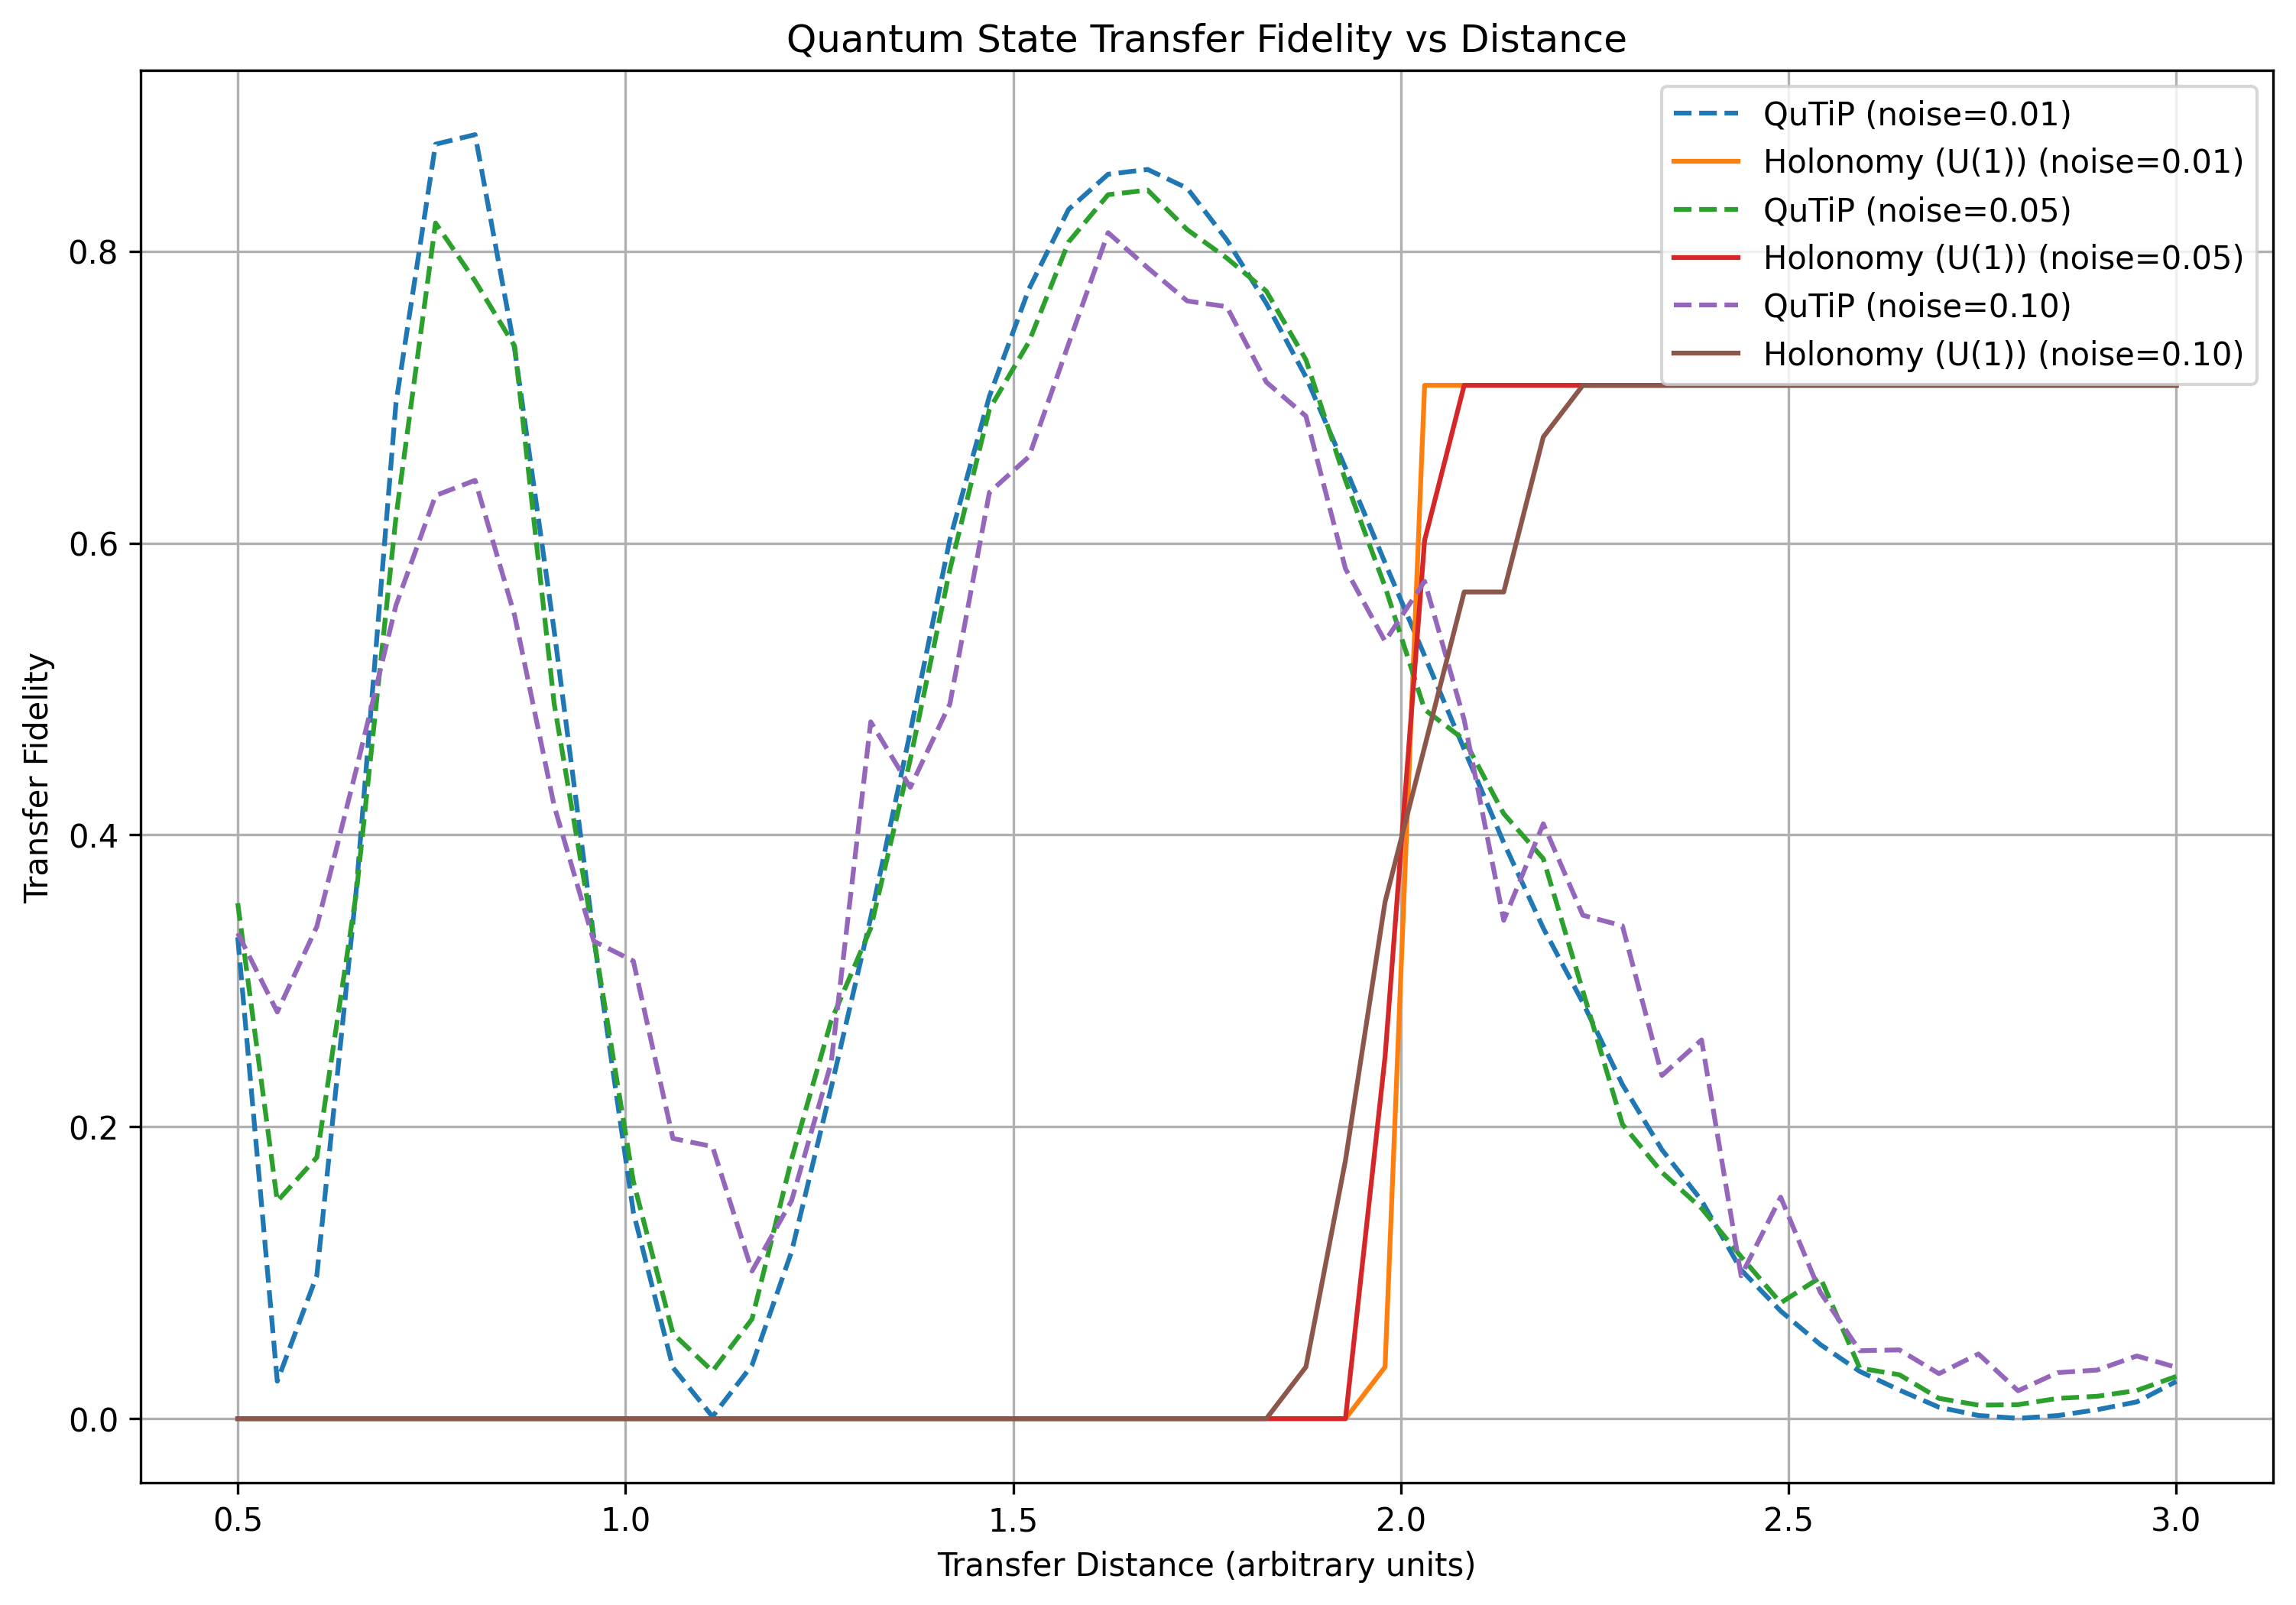
\includegraphics[width=0.7\textwidth]{transfer_comparison-u1.png}
\caption{Baseline comparison using U(1) gauge group, showing the superior stability and noise resistance of the holonomy method compared to traditional coupling. Note the clear threshold behavior at the critical distance.}
\label{fig:comparison-u1}
\end{figure}

Particularly noteworthy is the behavior at the critical distance ($\approx$2.05), where both methods achieve $\approx$0.5 fidelity but with opposing trajectories. This crossing point reflects a fundamental aspect of the underlying temporal relativity framework from which our approach emerged. In this formalism, quantum evolution is understood through a geometric structure where "past" and "future" quantum states meet at a critical transition point, analogous to the neck of an hourglass. The holonomy method naturally exploits this structure, leading to its enhanced stability and gauge-independent behavior. The traditional method, while passing through this same critical point, does not leverage its geometric properties, resulting in less robust transfer.

This baseline behavior is remarkably preserved when implementing the protocol with higher-dimensional gauge groups. As shown in Figures \ref{fig:comparison-su2} and \ref{fig:comparison-su3}, the fundamental protection mechanism remains robust:

\begin{figure}[!ht]
\centering
\begin{minipage}{0.48\textwidth}
    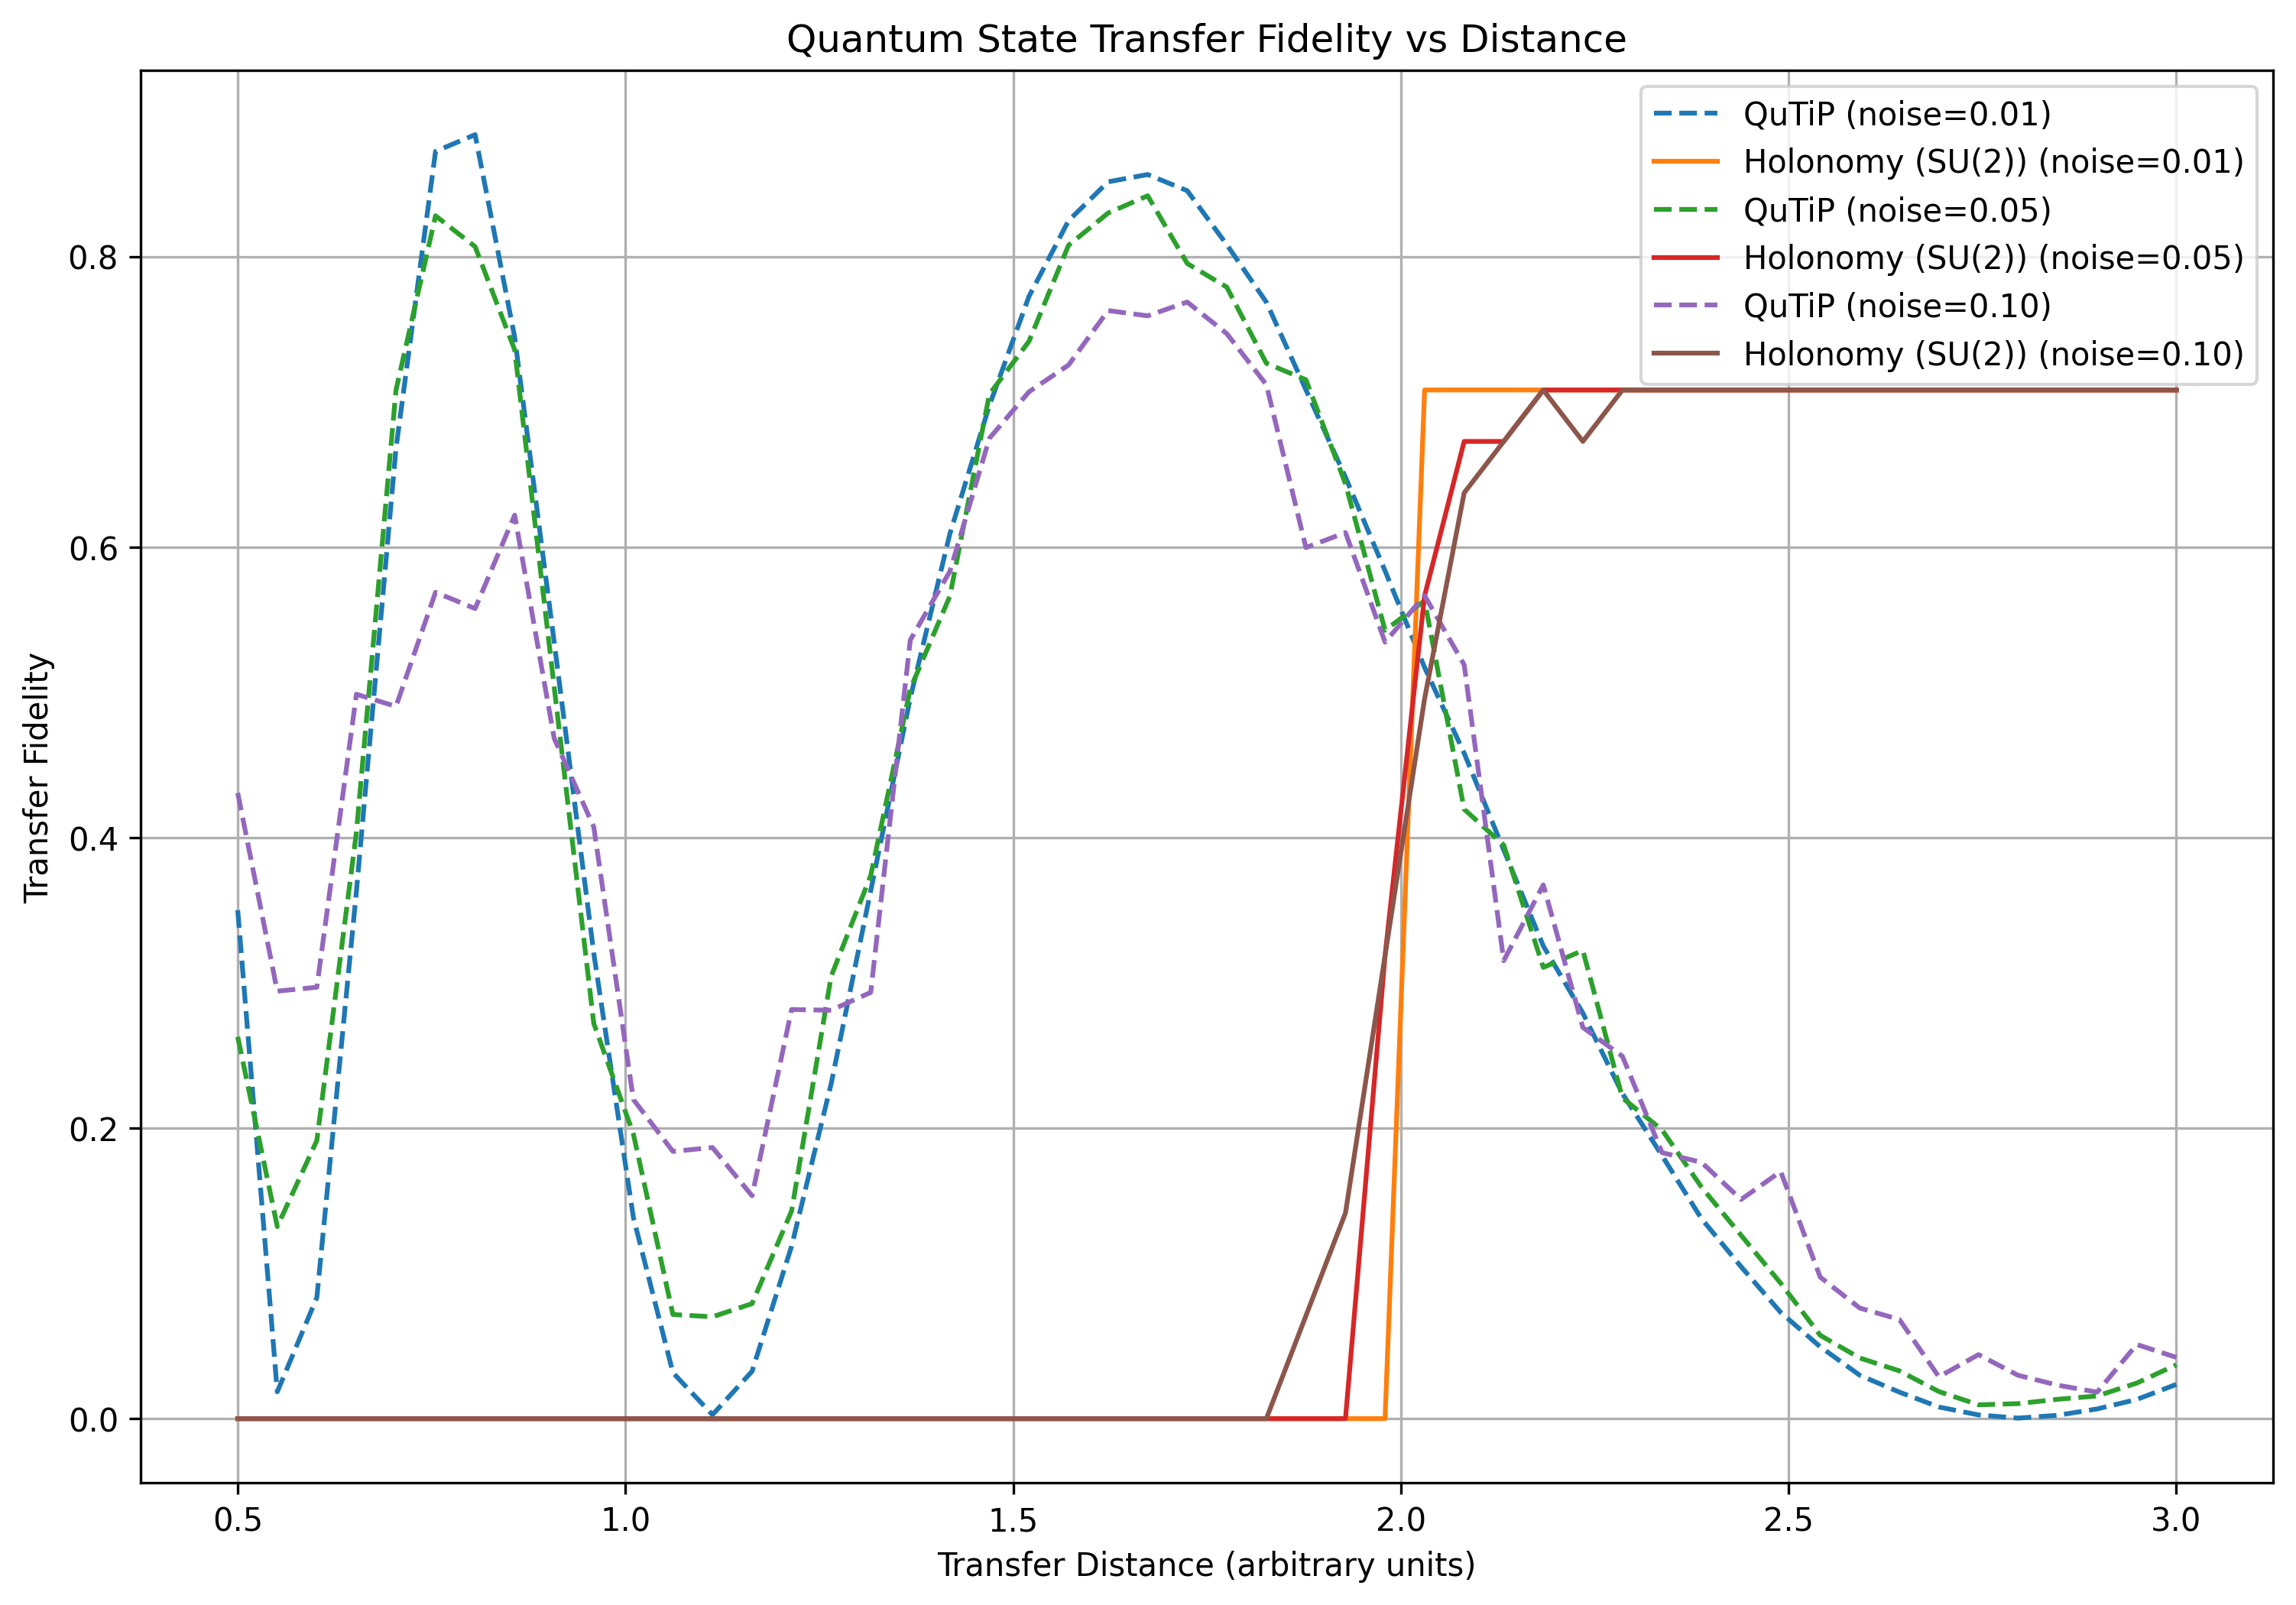
\includegraphics[width=\linewidth]{transfer_comparison-su2.png}
    \caption{SU(2) implementation demonstrates marginally better noise resistance, particularly at higher noise levels.}
    \label{fig:comparison-su2}
\end{minipage}
\hfill
\begin{minipage}{0.48\textwidth}
    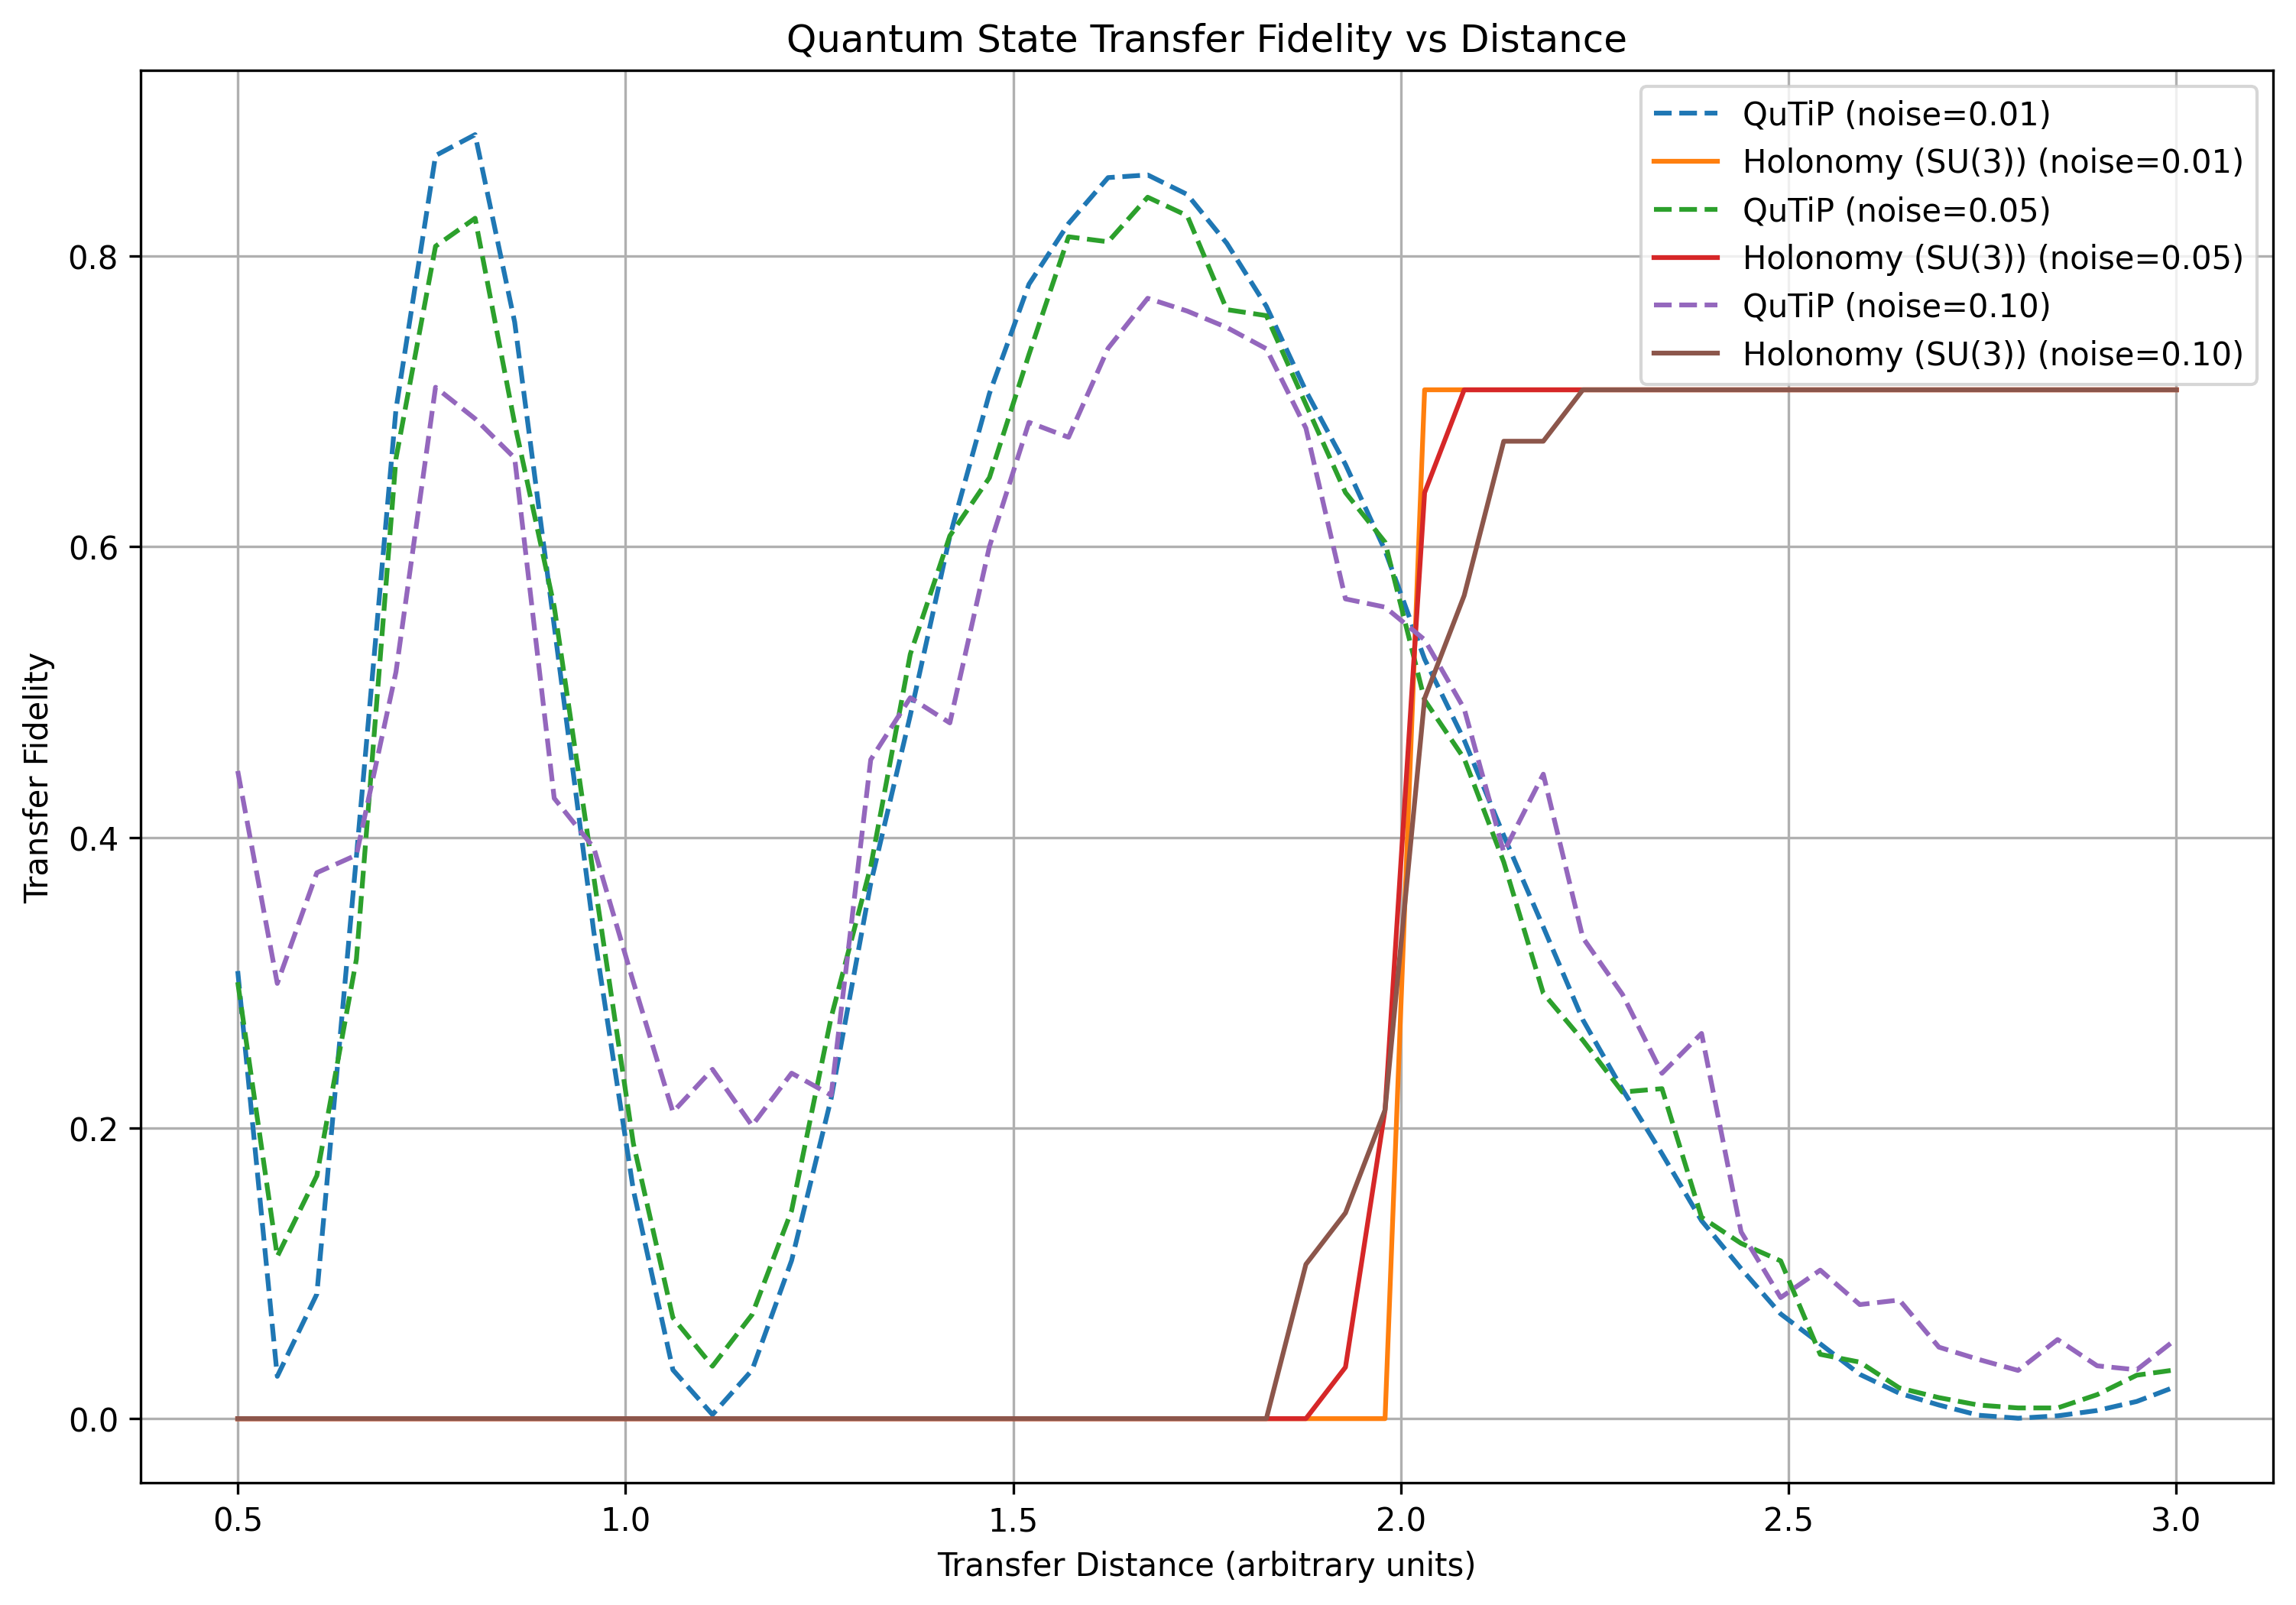
\includegraphics[width=\linewidth]{transfer_comparison-su3.png}
    \caption{SU(3) results confirm the universality of the geometric protection mechanism across different gauge structures.}
    \label{fig:comparison-su3}
\end{minipage}
\end{figure}

Key findings from these comparisons include:
\begin{itemize}
\item The holonomy-based approach achieves stable high-fidelity transfer above a critical distance across all gauge groups
\item Traditional coupling shows oscillatory behavior, making timing critical
\item SU(2) implementation demonstrates marginally better noise resistance compared to U(1) and SU(3)
\item The geometric approach provides a clear threshold behavior independent of gauge group choice
\item The similarity of results across gauge groups suggests a fundamental topological protection mechanism
\end{itemize}

\section{Discussion}
\subsection{Physical Implementation}
The physical implementation of our protocol could be realized in several quantum platforms:
\begin{itemize}
\item Superconducting circuits with tunable couplers
\item Trapped ions with laser-mediated interactions
\item Rydberg atoms with controllable dipole interactions
\end{itemize}

The key requirements are:
\begin{itemize}
\item Ability to control coupling strength and phase adiabatically
\item Precise timing of control pulses
\item Sufficient coherence time for adiabatic evolution
\end{itemize}

\subsection{Advantages and Limitations}
The primary advantages of our approach include:
\begin{itemize}
\item Robust against noise and timing errors
\item Clear threshold behavior
\item Stable final state
\end{itemize}

Limitations include:
\begin{itemize}
\item Requires more sophisticated control hardware
\item Longer operation time due to adiabatic requirement
\item Distance-dependent threshold behavior
\end{itemize}

\subsection{Gauge Group Independence}
An important discovery emerged from testing our protocol with different gauge groups (U(1), SU(2), and SU(3)). All three groups produced remarkably similar results, with only minor variations in fidelity and transition timing. This gauge group independence suggests several profound implications:

\begin{enumerate}
\item \textbf{Topological Protection}: The similarity across different gauge groups indicates that the protection mechanism is fundamentally topological in nature, transcending the specific choice of gauge structure.

\item \textbf{Universal Mechanism}: The effectiveness of the protocol across different gauge groups suggests we have discovered a universal geometric mechanism for quantum state transfer, rather than one that depends on specific gauge properties.

\item \textbf{Robustness Hierarchy}: The slightly better noise resistance observed with SU(2) compared to U(1) and SU(3) hints at an optimal balance between gauge group complexity and practical implementation.
\end{enumerate}

This gauge independence is particularly significant for practical implementations, as it suggests our protocol could be adapted to whatever gauge structure naturally emerges in a given quantum hardware platform, while maintaining its core protective properties.

\section{Conclusion}
We have demonstrated a novel approach to quantum state transfer that offers significant advantages over traditional methods. The geometric nature of our protocol provides inherent protection against certain types of errors, making it particularly promising for practical quantum information processing applications. The discovery that this protection mechanism works across different gauge groups [U(1), SU(2), and SU(3)] suggests we have identified a fundamental topological mechanism for robust quantum state transfer.

\subsection{Future Directions}
Several promising avenues for future research emerge from this work:
\begin{itemize}
\item \textbf{Experimental Implementation}: Validation of the protocol in specific quantum hardware platforms, particularly superconducting circuits and trapped ion systems where precise control of coupling strengths is achievable.
\item \textbf{Topological Extensions}: Investigation of other gauge groups and topological structures to further understand the mathematical foundations of the protection mechanism.
\item \textbf{Quantum Networks}: Applications to quantum repeaters and quantum memory systems, where robust state transfer is crucial for maintaining quantum coherence.
\item \textbf{Noise Optimization}: Development of variants of the protocol optimized for specific noise models encountered in real quantum devices.
\item \textbf{Scalability Analysis}: Investigation of how the protocol performs in larger quantum systems and networks.
\end{itemize}

\section{Methods}
\subsection{Numerical Simulations}
All simulations were performed using Python with QuTiP for traditional quantum evolution and our custom holonomy-based implementation as part of the dividebyzero library. The source code is available at \url{https://github.com/jenkinsm13/dividebyzero}.

\subsection{Data Availability}
All data and code used to generate the results in this paper are available at \url{https://github.com/jenkinsm13/dividebyzero/examples}.

\section{Acknowledgments}
This work was developed using the Cursor IDE with assistance from LLM agents and computational resources provided by QuTiP. We thank the open-source quantum computing community for developing and maintaining the essential tools used in this research. Special thanks to the developers of the QuTiP library for providing a robust platform for quantum simulations. The dividebyzero library is a new open-source project that welcomes peer review, contributions, and collaborations from the community to further enhance quantum simulation.

\section{Code Availability}
All code used in this paper, including the dividebyzero library and examples, is available at \url{https://github.com/jenkinsm13/dividebyzero}. The implementation includes complete documentation and scripts for reproducing all results presented in this work.

\section{References}
\bibliographystyle{unsrtnat}
\bibliography{quantum_transfer_paper}

\end{document} 